\chapter{Kính thiên văn}

\section{Lý thuyết trọng tâm}

\subsection{Công dụng và cấu tạo của kính thiên văn}

Kính thiên văn là những dụng cụ quang học bổ trợ cho mắt để nhìn những
thiên thể ở rất xa bằng cách tạo ảnh có góc trông lớn.

Kính thiên văn có hai bộ phận chính:
\begin{itemize}
	\item Vật kính $L_1$ là một thấu kính hội tụ có tiêu cự lớn (có thể đến hàng chục mét).
	\item Thị kính $L_2$ là một kính lúp dùng để quan sát ảnh của vật tạo bởi vật kính.
\end{itemize}

Khoảng cách $\text{O}_1\text{O}_2$ giữa hai kính có thể thay đổi được. 
\begin{center}
	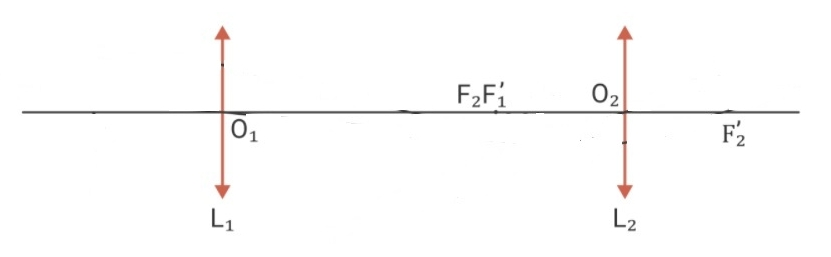
\includegraphics[scale=0.4]{../figs/VN11-PH-43-L-031-1-h54.jpg}
\end{center}

\subsection{Sự tạo ảnh bởi kính thiên văn}
\begin{center}
	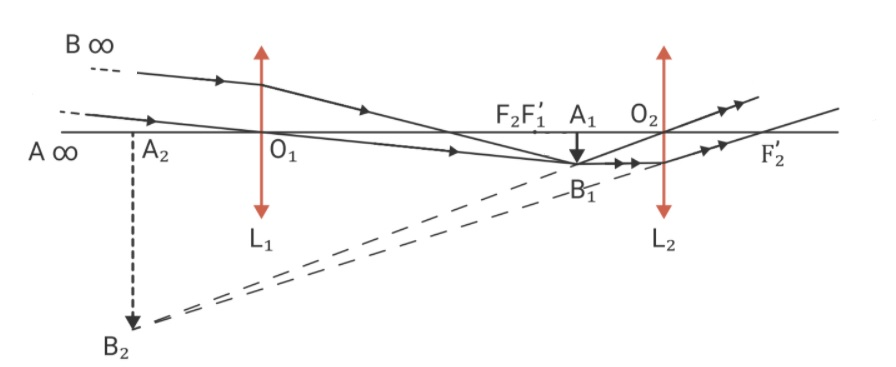
\includegraphics[scale=0.7]{../figs/VN11-PH-43-L-031-1-h56.jpg}
\end{center}
\begin{itemize}
	\item Vật kính có tác dụng tạo ảnh thật (ở vô cực) tại tiêu diện ảnh. 
	\item Thị kính giúp mắt quan sát ảnh này.
\end{itemize}

Ảnh của thiên thể tạo bởi kính thiên văn là ảnh ảo, ngược chiều với vật, có góc trông lớn hơn nhiều lần so với góc trông trực tiếp vật.

\subsection{Số bội giác của kính lúp khi ngắm chừng vô cực}
\begin{equation}
G_\infty=\dfrac{f_1}{f_2},
\end{equation}
trong đó,
\begin{itemize}
	\item $G_\infty$ là số bội giác của kính thiên văn khi ngắm chừng vô cực,
	\item $f_1$ là tiêu cự của vật kính,
	\item $f_2$ là tiêu cự của thị kính. 
\end{itemize}
Số bội giác của kính thiên văn trong điều kiện này không phụ thuộc vị trí đặt mắt sau thị kính. 


\section{Bài tập }
\begin{dang}{Ngắm chừng ở vô cực}
\end{dang}
\textbf{Phương pháp giải}

Số bội giác của kính lúp khi ngắm chừng vô cực: 
\begin{equation}
G_\infty=\dfrac{f_1}{f_2},
\end{equation}
trong đó,
\begin{itemize}
	\item $G_\infty$ là số bội giác của kính thiên văn khi ngắm chừng vô cực,
	\item $f_1$ là tiêu cự của vật kính,
	\item $f_2$ là tiêu cự của thị kính. 
\end{itemize}
Khoảng cách giữa vật kính và thị kính $$l=\text{O}_1\text{O}_2=f_1+f_2.$$


\viduii{2}{
Một kính thiên văn gồm vật kính có tiêu cự $f_1=120\ \text{cm}$ và thị kính có tiêu cự $f_2=5\ \text{cm}$. Độ bội giác của kính khi người mắt tốt quan sát Mặt Trăng trong trạng thái không điều tiết là
\begin{mcq}(4)
	\item 20.
	\item 24.
	\item 25.
	\item 30.
\end{mcq}}{
\begin{center}
	\textbf{Hướng dẫn giải:}
\end{center}

{ Đề bài cho khoảng cực cận $f_1=120\ \text{cm}, \ f_2=5\ \text{cm}$.
	
	
	$G_\infty=\dfrac{f_1}{f_2}=24$.
	
	\textbf{Đáp án: B.}
}
}
\viduii{2}{
Một kính thiên văn gồm vật kính có tiêu cự $f_1 =100\ \text{cm}$ và thị kính có tiêu cự $f_1 =5\ \text{cm}$. Độ bội giác của kính khi ngắm chừng vô cực và khoảng cách giữa hai kính khi người mắt tốt quan sát Mặt Trăng trong trạng thái không điều tiết là
\begin{mcq}(2)
	\item $G_\infty=20, \ l=500\ \text{cm}$.
	\item $G_\infty=20, \ l=150\ \text{cm}$.
	\item $G_\infty=20, \ l=95\ \text{cm}$.
	\item $G_\infty=20, \ l=105\ \text{cm}$.
\end{mcq}}{
\begin{center}
	\textbf{Hướng dẫn giải:}
\end{center}

{ Độ bội giác của kính khi ngắm chừng vô cực: $G_\infty=\dfrac{f_1}{f_2}=20$.
	
	Khoảng cách giữa hai kính khi người mắt tốt quan sát Mặt Trăng trong trạng thái không điều tiết là: $l=\text{O}_1\text{O}_2=f_1+f_2=l=105\ \text{cm}$.
	
	\textbf{Đáp án: D.}
}

}